\documentclass[journal,12pt,onecolumn]{IEEEtran}
\usepackage{cite}
\usepackage{graphicx}
\usepackage{amsmath,amssymb,amsfonts,amsthm}
\usepackage{algorithmic}
\usepackage{graphicx}
\usepackage{textcomp}
\usepackage{xcolor}
\usepackage{txfonts}
\usepackage{listings}
\usepackage{enumitem}
\usepackage{mathtools}
\usepackage{gensymb}
\usepackage{comment}
\usepackage[breaklinks=true]{hyperref}
\usepackage{tkz-euclide} 
\usepackage{listings}
\usepackage{gvv}                                        
\usepackage[latin1]{inputenc} 
\usetikzlibrary{arrows.meta, positioning}
\usepackage{xparse}
\usepackage{color}                                            
\usepackage{array}                                            
\usepackage{longtable}                                       
\usepackage{calc}                                             
\usepackage{multirow}
\usepackage{multicol}
\usepackage{hhline}                                           
\usepackage{ifthen}                                           
\usepackage{lscape}
\usepackage{tabularx}
\usepackage{array}
\usepackage{float}
\newtheorem{theorem}{Theorem}[section]
\newtheorem{problem}{Problem}
\newtheorem{proposition}{Proposition}[section]
\newtheorem{lemma}{Lemma}[section]
\newtheorem{corollary}[theorem]{Corollary}
\newtheorem{example}{Example}[section]
\newtheorem{definition}[problem]{Definition}
\newcommand{\BEQA}{\begin{eqnarray}}
\newcommand{\EEQA}{\end{eqnarray}}
\usepackage{float}
\theoremstyle{remark}
\usepackage{circuitikz}
\usepackage{tikz}
\title{GG: GEOLOGY AND GEOPHYSICS}
\author{EE25BTECH11032- KARTIK LAHOTI}
\begin{document}

\maketitle

\begin{enumerate}

\item If '$\rightarrow$' denotes increasing order of intensity, then the meaning of the words $\brak{\text{simmer} \rightarrow \text{seethe} \rightarrow \text{smolder}}$ is analogous to $\brak{\text{break} \rightarrow \text{raze} \rightarrow \rule{3cm}{0.15mm}}$. Which one of the given options is appropriate to fill the blank?
\begin{enumerate}
    \begin{multicols}{4}
    \item obfuscate
    \item obliterate
    \item fracture
    \item fissure
    \end{multicols}
\end{enumerate}
\hfill{\brak{\text{GATE GG 2025}}}

\item In a locality, the houses are numbered in the following way:
The house-numbers on one side of a road are consecutive odd integers starting from $301$, while the house-numbers on the other side of the road are consecutive even numbers starting from $302$. The total number of houses is the same on both sides of the road.
If the difference of the sum of the house-numbers between the two sides of the road is $27$, then the number of houses on each side of the road is
\begin{enumerate}
    \begin{multicols}{4}
    \item $27$
    \item $52$
    \item $54$
    \item $26$
    \end{multicols}
\end{enumerate}
\hfill{\brak{\text{GATE GG 2025}}}

\item For positive integers $p$ and $q$, with $\frac{p}{q} \neq 1\,, \brak{\frac{p}{q}}^{\frac{p}{q}} = p^{\brak{\frac{p}{q}-1}}$. Then,
\begin{enumerate}
    \begin{multicols}{2}
    \item $q^p = p^q$
    \item $q^p = p^{2q}$
    \item $\sqrt{q} = \sqrt{p}$
    \item $\sqrt[p]{q} = \sqrt[q]{p}$
    \end{multicols}
\end{enumerate}
\hfill{\brak{\text{GATE GG 2025}}}

\item Which one of the given options is a possible value of $x$ in the following sequence?
$3, 7, 15,x,63, 127, 255$
\begin{enumerate}
    \begin{multicols}{4}
    \item $35$
    \item $40$
    \item $45$
    \item $31$
    \end{multicols}
\end{enumerate}
\hfill{\brak{\text{GATE GG 2025}}}

\item On a given day, how many times will the second-hand and the minute-hand of a clock cross each other during the clock time $12\colon05\colon00$ hours to $12\colon55\colon00$ hours?
\begin{enumerate}
    \begin{multicols}{4}
    \item $51$
    \item $49$
    \item $50$
    \item $55$
    \end{multicols}
\end{enumerate}
\hfill{\brak{\text{GATE GG 2025}}}

\item In the given text, the blanks are numbered $\brak{i}-\brak{iv}$. Select the best match for all the blanks.
From the ancient Athenian arena to the modern Olympic stadiums, athletics \rule{0.5cm}{0.15mm}$\brak{i}$\rule{0.5cm}{0.15mm} the potential for a spectacle. The crowd \rule{0.5cm}{0.15mm}$\brak{ii}$\rule{0.5cm}{0.15mm} with bated breath as the Olympian artist twists his body, stretching the javelin behind him. Twelve strides in, he begins to cross-step. Six cross-steps \rule{0.5cm}{0.15mm}$\brak{iii}$\rule{0.5cm}{0.15mm} in an abrupt stop on his left foot. As his body \rule{0.5cm}{0.15mm}$\brak{iv}$\rule{0.5cm}{0.15mm} like a door turning on a hinge, the javelin is launched skyward at a precise angle.
\begin{enumerate}
    \item \brak{i} hold \brak{ii} waits \brak{iii} culminates \brak{iv} pivot
    \item \brak{i} holds \brak{ii} wait \brak{iii} culminates \brak{iv} pivot
    \item \brak{i} hold \brak{ii} wait \brak{iii} culminate \brak{iv} pivots
    \item \brak{i} holds \brak{ii} waits \brak{iii} culminate \brak{iv} pivots
\end{enumerate}
\hfill{\brak{\text{GATE GG 2025}}}

\item Three distinct sets of indistinguishable twins are to be seated at a circular table that has $8$ identical chairs. Unique seating arrangements are defined by the relative positions of the people. How many unique seating arrangements are possible such that each person is sitting next to their twin?
\begin{enumerate}
    \begin{multicols}{4}
    \item $12$
    \item $14$
    \item $10$
    \item $28$
    \end{multicols}
\end{enumerate}
\hfill{\brak{\text{GATE GG 2025}}}

\item The chart given below compares the Installed Capacity \brak{MW} of four power generation technologies, T1, T2, T3, and T4, and their Electricity Generation \brak{MWh} in a time of $1000$ hours $\brak{h}$.
\begin{figure}[H]
    \centering
    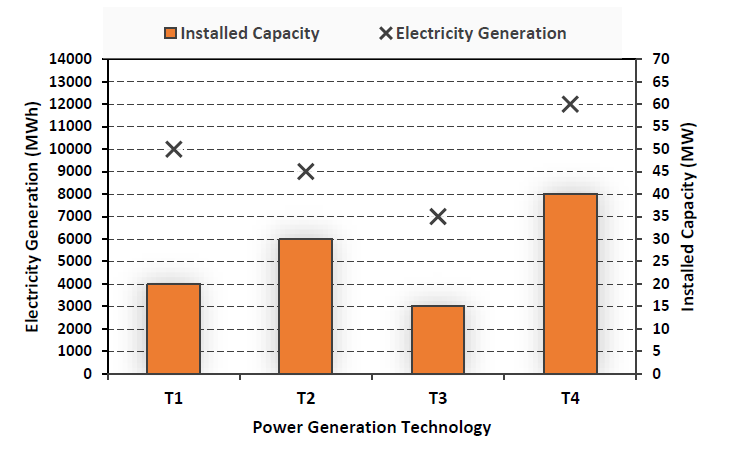
\includegraphics[width=0.8\columnwidth]{Figs/fig_1.png}
    \caption{Q.8.}
    \label{fig:q8}
\end{figure}
The Capacity Factor of a power generation technology is:
$$ \frac{\text{Electricity Generation \brak{MWh}}}{\text{Installed Capacity \brak{MW}} \times 1000 \text{ \brak{h}}} $$
Which one of the given technologies has the highest Capacity Factor?
\begin{enumerate}
    \begin{multicols}{4}
    \item T1
    \item T2
    \item T3
    \item T4
    \end{multicols}
\end{enumerate}
\hfill{\brak{\text{GATE GG 2025}}}

\item In the $4 \times 4$ array shown below, each cell of the first three columns has either a cross $\brak{X}$ or a number, as per the given rule.
\begin{figure}[H]
    \centering
    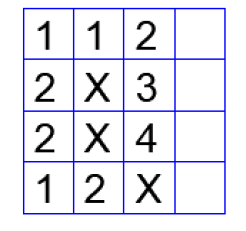
\includegraphics[width=0.2\columnwidth]{Figs/fig_2.png}
    \caption{Q.9.}
    \label{fig:q9}
\end{figure}
Rule $\colon$ The number in a cell represents the count of crosses around its immediate neighboring cells \brak{\text{left, right, top, bottom, diagonals}}.
As per this rule, the maximum number of crosses possible in the empty column is
\begin{enumerate}
    \begin{multicols}{4}
    \item $0$
    \item $1$
    \item $2$
    \item $3$
    \end{multicols}
\end{enumerate}
\hfill{\brak{\text{GATE GG 2025}}}

\item During a half-moon phase, the Earth-Moon-Sun form a right triangle. If the Moon-Earth-Sun angle at this half-moon phase is measured to be $89.85\degree$, the ratio of the Earth-Sun and Earth-Moon distances is closest to
\begin{enumerate}
    \begin{multicols}{4}
    \item $328$
    \item $382$
    \item $238$
    \item $283$
    \end{multicols}
\end{enumerate}
\hfill{\brak{\text{GATE GG 2025}}}

\item The Earth's magnetic field originates from convection in which one of the following layers?
\begin{enumerate}
    \begin{multicols}{4}
    \item Inner core
    \item Outer core
    \item Lithosphere
    \item Asthenosphere
    \end{multicols}
\end{enumerate}
\hfill{\brak{\text{GATE GG 2025}}}

\item Which one of the following logging tools is used to measure the diameter of a borehole?
\begin{enumerate}
    \begin{multicols}{4}
    \item Caliper
    \item Gamma Ray
    \item Spontaneous Potential
    \item Neutron
    \end{multicols}
\end{enumerate}
\hfill{\brak{\text{GATE GG 2025}}}

\item The given figure depicts an array used in DC resistivity surveys, where the current electrodes are denoted by $C1$ and $C2$, and potential electrodes by $P1$ and $P2$. If all the electrodes are equally spaced, then the given array corresponds to which one of the following configurations?
\begin{figure}[H]
    \centering
    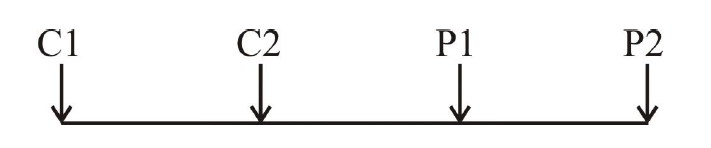
\includegraphics[width=0.6\columnwidth]{Figs/fig_3.png}
    \caption{Q.13.}
    \label{fig:q13}
\end{figure}
\begin{enumerate}
    \begin{multicols}{4}
    \item Wenner
    \item Schlumberger
    \item Dipole-Dipole
    \item Pole-Pole
    \end{multicols}
\end{enumerate}
\hfill{\brak{\text{GATE GG 2025}}}

\item Which one of the following is an ultramafic rock?
\begin{enumerate}
    \begin{multicols}{4}
    \item Granite
    \item Gabbro
    \item Dunite
    \item Basalt
    \end{multicols}
\end{enumerate}
\hfill{\brak{\text{GATE GG 2025}}}

\item Gold is being produced from which one of the following mines in India?
\begin{enumerate}
    \begin{multicols}{4}
    \item Baula
    \item Hutti
    \item Dariba
    \item Jaduguda
    \end{multicols}
\end{enumerate}
\hfill{\brak{\text{GATE GG 2025}}}

\item Which of the following hydrocarbon fields is/are located in the western offshore of India?
\begin{enumerate}
    \begin{multicols}{4}
    \item Tapti
    \item Lakwa
    \item Ravva
    \item Panna
    \end{multicols}
\end{enumerate}
\hfill{\brak{\text{GATE GG 2025}}}

\item A cylindrical sample of granite $\brak{\text{diameter} = 54.7 \text{ mm; length} = 137 \text{ mm}}$ shows a linear relationship between axial stress and axial strain under uniaxial compression up to the peak stress level at which the specimen fails. If the uniaxial compressive strength of this sample is $200\,MPa$ and the axial strain corresponding to this peak stress is $0.005$, the Young's modulus of the sample in $GPa$ is \rule{3cm}{0.15mm} \brak{\text{in integer}}.
\hfill{\brak{\text{GATE GG 2025}}}

\item The given figure shows the ray path of a P-wave propagating through the Earth. Choose the CORRECT P-phase corresponding to the ray path.
\begin{figure}[H]
    \centering
    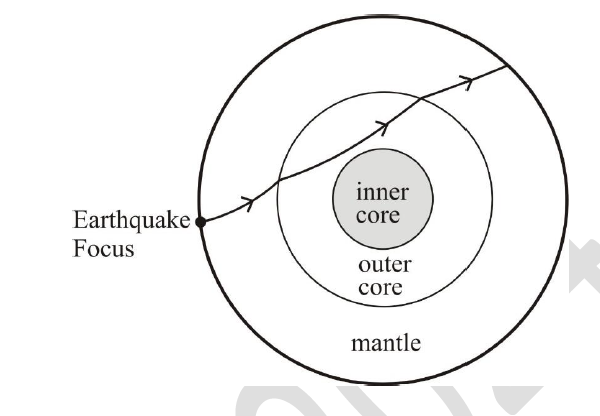
\includegraphics[width=0.4\columnwidth]{Figs/fig_4.png}
    \caption{Q.18.}
    \label{fig:q18}
\end{figure}
\begin{enumerate}
    \begin{multicols}{4}
    \item PcP
    \item PKP
    \item PPP
    \item PmP
    \end{multicols}
\end{enumerate}
\hfill{\brak{\text{GATE GG 2025}}}

\item Match the geophysical methods in Group-$I$ with their associated physical properties in Group-$II$.

        \begin{multicols}{2}
            \underline{\textbf{Group $I$}}
            \begin{enumerate}[start =16]
                \item Magnetic
                \item Gravity
                \item Magnetotelluric
                \item Induced Polarization
            \end{enumerate}

            \columnbreak

            \underline{\textbf{Group $II$}}
            \begin{enumerate}
                \item Chargeability
                \item Electrical conductivity
                \item Susceptibility
                \item Density                
            \end{enumerate}
        \end{multicols}
\begin{enumerate}
    \begin{multicols}{2}
        \item P-$3$, Q-$4$, R-$2$, S-$1$
        \item P-$3$, Q-$4$, R-$1$, S-$2$
        \item P-$4$, Q-$3$, R-$2$, S-$1$
        \item P-$2$, Q-$1$, R-$4$, S-$3$
    \end{multicols}
\end{enumerate}
\hfill{\brak{\text{GATE GG 2025}}}

\item The number of planes of symmetry in a tetrahedron is
\begin{enumerate}
    \begin{multicols}{4}
    \item $9$
    \item $6$
    \item $4$
    \item $3$
    \end{multicols}
\end{enumerate}
\hfill{\brak{\text{GATE GG 2025}}}

\item Which of the following Epochs belong\brak{s} to the Quaternary Period?
\begin{enumerate}
    \begin{multicols}{4}
    \item Holocene
    \item Pleistocene
    \item Pliocene
    \item Miocene
    \end{multicols}
\end{enumerate}
\hfill{\brak{\text{GATE GG 2025}}}

\item Which one or more of the following minerals shows $O\colon Si$ ratio of $4\colon1$ in its silicate structure?
\begin{enumerate}
    \begin{multicols}{4}
    \item Olivine
    \item Quartz
    \item Diopside
    \item Albite
    \end{multicols}
\end{enumerate}
\hfill{\brak{\text{GATE GG 2025}}}

\item Which of the following rock structures is/are fold\brak{s}?
\begin{enumerate}
    \begin{multicols}{4}
    \item Antiform
    \item Horst
    \item Syncline
    \item Synform
    \end{multicols}
\end{enumerate}
\hfill{\brak{\text{GATE GG 2025}}}

\item Assume heat producing elements are uniformly distributed within a $16\,km$ thick layer in the crust in a heat flow province. Given that the surface heat flow and reduced heat flow are $54\,mW/m^2$ and $22\,mW/m^2$, respectively, the radiogenic heat production in the given crustal layer in $\mu\,W/m^3$ is \rule{3cm}{0.15mm} \brak{\text{in integer}}.
\hfill{\brak{\text{GATE GG 2025}}}

\item A confined aquifer with a uniform saturated thickness of $10\,m$ has hydraulic conductivity of $10^{-2}\,cm/s$ cm/s. Considering a steady flow, the transmissivity of the aquifer in $m^2/day$ is \rule{3cm}{0.15mm} \brak{\text{rounded off to one decimal place}}.
\hfill{\brak{\text{GATE GG 2025}}}

\item A current of $2$ A passes through a cylindrical rod with uniform cross-sectional area of $4\,m^2$ and resistivity of $100\,\ohm-m$. The magnitude of the electric field $\brak{E}$ measured along the length of the rod in $V/m$ is \rule{3cm}{0.15mm} \brak{\text{in integer}}.
\hfill{\brak{\text{GATE GG 2025}}}

\item Which one of the following lineations can be observed on a foliation with an attitude $210\degree, 40\degree\,NW$ ?
\begin{enumerate}
    \begin{multicols}{4}
    \item $40\degree \rightarrow 300\degree$
    \item $40\degree \rightarrow 040\degree$
    \item $40\degree \rightarrow 220\degree$
    \item $40\degree \rightarrow 350\degree$
    \end{multicols}
\end{enumerate}
\hfill{\brak{\text{GATE GG 2025}}}

\item Match the minerals in Group-$I$ with the corresponding cleavage types in Group-$II$.

\begin{multicols}{2}
            \underline{\textbf{Group $I$}}
            \begin{enumerate}[start =16]
                \item Diopside
                \item Galena
                \item Calcite
                \item Fluorite
            \end{enumerate}

            \columnbreak

            \underline{\textbf{Group $II$}}
            \begin{enumerate}
                \item Cubic
                \item Octahedral
                \item Prismatic
                \item Rhombohedral
            \end{enumerate}
        \end{multicols}
\begin{enumerate}
    \begin{multicols}{2}
        \item P-$3$, Q-$2$, R-$4$, S-$1$
        \item P-$4$, Q-$3$, R-$1$, S-$2$
        \item P-$3$, Q-$1$, R-$4$, S-$2$
        \item P-$4$, Q-$1$, R-$2$, S-$3$
    \end{multicols}
\end{enumerate}
\hfill{\brak{\text{GATE GG 2025}}}

\item The composition of which one of the following reservoirs closely matches with that of iron meteorites?
\begin{enumerate}
    \begin{multicols}{4}
    \item Primitive Mantle
    \item Earth's Core
    \item Depleted Mantle
    \item Bulk Silicate Earth
    \end{multicols}
\end{enumerate}
\hfill{\brak{\text{GATE GG 2025}}}

\item Match the microstructures in Group-$I$ with their characteristics in Group-$II$.

\begin{multicols}{2}
            \underline{\textbf{Group $I$}}
            \begin{enumerate}[start =16]
                \item Core-mantle
                \item Decussate
                \item Spherulite
                \item Millipede
            \end{enumerate}

            \columnbreak

            \underline{\textbf{Group $II$}}
            \begin{enumerate}
                \item Radiating fibrous aggregate of K-feldspar with or without quartz
                \item Large strained mineral grains surrounded by fine-grained, recrystallized grains
                \item Inclusion trails in a porphyroblast curves into the matrix foliation by developing concave outward pattern
                \item Randomly oriented mineral grains dominated by crystal faces, such as in sheet silicates
            \end{enumerate}
        \end{multicols}

\begin{enumerate}
    \begin{multicols}{2}
        \item P-$2$, Q-$3$, R-$4$, S-$1$
        \item P-$3$, Q-$4$, R-$1$, S-$2$
        \item P-$2$, Q-$4$, R-$1$, S-$3$
        \item P-$4$, Q-$2$, R-$3$, S-$1$
    \end{multicols}
\end{enumerate}
\hfill{\brak{\text{GATE GG 2025}}}

\item Which one among the following is the least abundant sedimentary rock in the stratigraphic record?
\begin{enumerate}
    \begin{multicols}{4}
    \item Sandstone
    \item Limestone
    \item Conglomerate
    \item Shale
    \end{multicols}
\end{enumerate}
\hfill{\brak{\text{GATE GG 2025}}}

\item Which one of the following sequences of index minerals correctly represents the order of increasing metamorphic grade during regional metamorphism of siliceous dolomitic limestones?
\begin{enumerate}
    \item Tremolite $\rightarrow$ Diopside $\rightarrow$ Talc
    \item Diopside $\rightarrow$ Tremolite $\rightarrow$ Forsterite
    \item Talc $\rightarrow$ Tremolite $\rightarrow$ Diopside
    \item Talc $\rightarrow$ Forsterite $\rightarrow$ Tremolite
\end{enumerate}
\hfill{\brak{\text{GATE GG 2025}}}

\item Which one among the following is the oldest horse genus?
\begin{enumerate}
    \begin{multicols}{4}
    \item Orohippus
    \item Mesohippus
    \item Merychippus
    \item Pliohippus
    \end{multicols}
\end{enumerate}
\hfill{\brak{\text{GATE GG 2025}}}

\item The measured plate velocity is maximum \brak{\text{in International Terrestrial Reference Frame}} at which one of the following locations on the Indian Plate?
\begin{enumerate}
    \begin{multicols}{4}
    \item Leh
    \item Delhi
    \item Bengaluru
    \item Maldives
    \end{multicols}
\end{enumerate}
\hfill{\brak{\text{GATE GG 2025}}}

\item Which one of the following textures is called the chalcopyrite disease?
\begin{enumerate}
    \item Chalcopyrite blebs in sphalerite
    \item Sphalerite stars in chalcopyrite
    \item Chalcopyrite lamellae in bornite
    \item Bornite lamellae in chalcopyrite
\end{enumerate}
\hfill{\brak{\text{GATE GG 2025}}}

\item Which one of the following is the correct arrangement of volcanics from the oldest to the youngest?
\begin{enumerate}
    \item Bijli $\rightarrow$ Rajmahal $\rightarrow$ Malani $\rightarrow$ Deccan
    \item Malani $\rightarrow$ Bijli $\rightarrow$ Deccan $\rightarrow$ Rajmahal
    \item Bijli $\rightarrow$ Malani $\rightarrow$ Rajmahal $\rightarrow$ Deccan
    \item Malani $\rightarrow$ Rajmahal $\rightarrow$ Bijli $\rightarrow$ Deccan
\end{enumerate}
\hfill{\brak{\text{GATE GG 2025}}}

\item Which of the following types of deposits is/are formed by fractional crystallization of magma?
\begin{enumerate}
    \begin{multicols}{2}
    \item Komatiite hosted $Ni-Cu$
    \item Peridotite hosted $Cr$
    \item Leucogranite hosted $U$
    \item Anorthosite hosted $Ti-Fe$
    \end{multicols}
\end{enumerate}
\hfill{\brak{\text{GATE GG 2025}}}

\item Which of the following sedimentary basins is/are producing hydrocarbon commercially?
\begin{enumerate}
    \begin{multicols}{4}
    \item Ganga
    \item Krishna-Godavari
    \item Kerala-Konkan
    \item Cauvery
    \end{multicols}
\end{enumerate}
\hfill{\brak{\text{GATE GG 2025}}}

\item Which of the following bivalves is/are swimmers?
\begin{enumerate}
    \begin{multicols}{4}
    \item Aspergillum
    \item Lima
    \item Tellina
    \item Pecten
    \end{multicols}
\end{enumerate}
\hfill{\brak{\text{GATE GG 2025}}}

\item Which of the following structures is/are associated with duplexes in fold-thrust belts?
\begin{enumerate}
    \begin{multicols}{4}
    \item Roof thrust
    \item Floor thrust
    \item Imbricate fan
    \item Horses
    \end{multicols}
\end{enumerate}
\hfill{\brak{\text{GATE GG 2025}}}

\item Which of the following statements is/are CORRECT?
\begin{enumerate}
    \item Karst topography is formed in limestone terrains
    \item Fjords are formed by aeolian activities
    \item Oxbow lakes are formed in fluvial environments
    \item Ventifacts are formed by glaciers
\end{enumerate}
\hfill{\brak{\text{GATE GG 2025}}}

\item Consider the solubility product of barite $\brak{BaSO_4}$ at $25\degree\,C \text{ and }1$ bar to be $10^{-10}$. If the activities of $Ba^{2+}$ and $SO_4^{2-}$ ions are $0.5 \times 10^{-5}$ and $10^{-X}$, respectively, then the absolute value of '$X$' is \rule{3cm}{0.15mm} \brak{\text{rounded off to one decimal place}}.
\hfill{\brak{\text{GATE GG 2025}}}

\item The support pressure of $20\,kPa$ is required to stabilize the loose blocks of the Excavation Disturbed Zone \brak{EDZ} at the crown of a circular tunnel with horizontal axis. The EDZ is to be stabilized by inserting rock bolts vertically into the roof. If the working capacity of a bolt is $160\,kN$ , the area of the roof supported by a single bolt in $m^2$ is \rule{3cm}{0.15mm} \brak{\text{in integer}}.
\hfill{\brak{\text{GATE GG 2025}}}

\item The areas of drainage basins A and B are $25\,km^2$ and $50\,km^2$, respectively. The total length of drainages of all orders in basin A is $20\,km$ . If both the basins have the same drainage density, the total length of drainages of all orders in basin B in km is \rule{3cm}{0.15mm} \brak{\text{in integer}}.
\hfill{\brak{\text{GATE GG 2025}}}

\item Match the stratigraphic units in Group-$I$ with the sedimentary basins in Group-$II$.

\begin{multicols}{2}
            \underline{\textbf{Group $I$}}
            \begin{enumerate}[start =16]
                \item Ramgundam Sandstone
                \item Raipur Formation
                \item Bagalkot Group
                \item Sonia Sandstone
            \end{enumerate}

            \columnbreak

            \underline{\textbf{Group $II$}}
            \begin{enumerate}
                \item Chhattisgarh
                \item Kaladgi
                \item Marwar
                \item Godavari
            \end{enumerate}
        \end{multicols}
\begin{enumerate}
    \begin{multicols}{2}
        \item P-$2$, Q-$1$, R-$4$, S-$3$
        \item P-$4$, Q-$1$, R-$2$, S-$3$
        \item P-$4$, Q-$3$, R-$2$, S-$1$
        \item P-$1$, Q-$4$, R-$3$, S-$2$
    \end{multicols}
\end{enumerate}
\hfill{\brak{\text{GATE GG 2025}}}

\item Which one of the following openings is a type of decline in underground mines?
\begin{enumerate}
    \begin{multicols}{4}
    \item Crosscut
    \item Winze
    \item Spiral tunnel
    \item Drift
    \end{multicols}
\end{enumerate}
\hfill{\brak{\text{GATE GG 2025}}}

\item Which one of the following optic signs is CORRECT for a mineral with the given centered optic axis figure?
\begin{figure}[H]
    \centering
    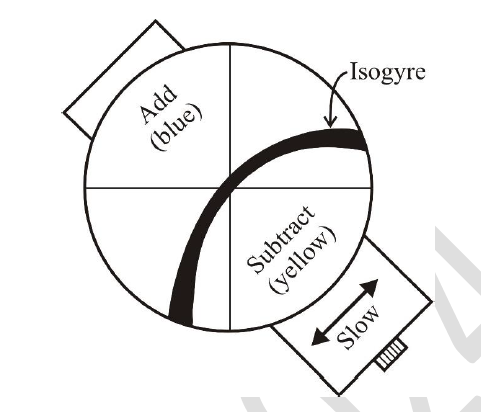
\includegraphics[width=0.4\columnwidth]{Figs/fig_5.png}
    \caption{Q.47}
    \label{fig:q47}
\end{figure}
\begin{enumerate}
    \begin{multicols}{4}
    \item Uniaxial positive
    \item Biaxial positive
    \item Uniaxial negative
    \item Biaxial negative
    \end{multicols}
\end{enumerate}
\hfill{\brak{\text{GATE GG 2025}}}

\item Match the following invertebrates in Group-$I$ with their morphological features in Group-$II$.

\begin{multicols}{2}
            \underline{\textbf{Group $I$}}
            \begin{enumerate}[start =16]
                \item Trilobite
                \item Brachiopod
                \item Bivalve
                \item Echinoid
            \end{enumerate}

            \columnbreak

            \underline{\textbf{Group $II$}}
            \begin{enumerate}
                \item Periproct
                \item Hypostome
                \item Deltidial plate
                \item Lunule
            \end{enumerate}
        \end{multicols}
\begin{enumerate}
    \begin{multicols}{2}
        \item P-$2$, Q-$4$, R-$1$, S-$3$
        \item P-$2$, Q-$3$, R-$4$, S-$1$
        \item P-$4$, Q-$3$, R-$1$, S-$2$
        \item P-$3$, Q-$2$, R-$4$, S-$1$
    \end{multicols}
\end{enumerate}
\hfill{\brak{\text{GATE GG 2025}}}

\item During high-temperature metamorphism of pelites, which one of the following mineral reactions represents the second sillimanite isograd?
\begin{enumerate}
    \item Muscovite $+$ Quartz $=$ Sillimanite $+$ K-feldspar $+ H_2O$
    \item Staurolite $+$ Quartz $=$ Garnet $+$ Sillimanite $+ H_2O$
    \item Staurolite $+$ Muscovite $+$ Quartz $=$ Garnet $+$ Biotite $+$ Sillimanite $+ H_2O$
    \item Kyanite $=$ Sillimanite
\end{enumerate}
\hfill{\brak{\text{GATE GG 2025}}}

\item Which one of the following represents deviatoric stress in a $2D$ stress Mohr Circle?
\begin{enumerate}
    \begin{multicols}{4}
    \item Radius
    \item Center
    \item Pole
    \item Diameter
    \end{multicols}
\end{enumerate}
\hfill{\brak{\text{GATE GG 2025}}}

\item In the fold profile section shown in the figure, $1$ and $3$ are the oldest and the youngest stratigraphic units, respectively. Which one of the following fold descriptions CORRECTLY matches the asymmetric fold shown in the given figure?
\begin{figure}[H]
    \centering
    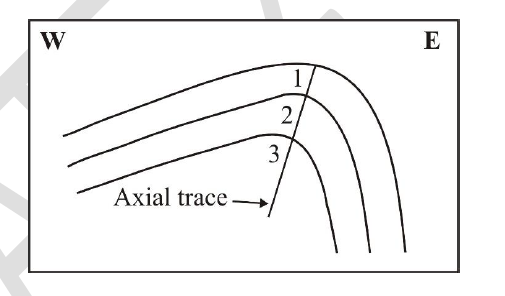
\includegraphics[width=0.5\columnwidth]{Figs/fig_6.png}
    \caption{Q.51.}
    \label{fig:q51}
\end{figure}
\begin{enumerate}
    \begin{multicols}{2}
    \item Antiform facing east
    \item Synform facing east
    \item Antiform facing west
    \item Synform facing west
    \end{multicols}
\end{enumerate}
\hfill{\brak{\text{GATE GG 2025}}}

\item If '$X$' represents the initial composition of a melt, which one of the trends indicated by arrows in the schematic diagram corresponds to the evolution of the residual melt composition during crystallization of diopside?
\begin{figure}[H]
    \centering
    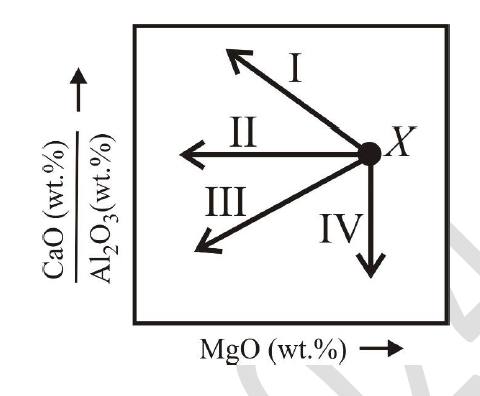
\includegraphics[width=0.5\columnwidth]{Figs/fig_7.png}
    \caption{Q.52.}
    \label{fig:q52}
\end{figure}
\begin{enumerate}
    \begin{multicols}{4}
    \item I
    \item II
    \item III
    \item IV
    \end{multicols}
\end{enumerate}
\hfill{\brak{\text{GATE GG 2025}}}

\item Match the following copper deposits in Group-$I$ with their host rocks in Group-$II$.
\begin{multicols}{2}
            \underline{\textbf{Group $I$}}
            \begin{enumerate}[start =16]
                \item Khetri
                \item Mosabani
                \item Malanjkhand
                \item Kalyadi
            \end{enumerate}

            \columnbreak

            \underline{\textbf{Group $II$}}
            \begin{enumerate}
                \item Chlorite-biotite schist and soda-granite
                \item Garnetiferous chlorite schist
                \item Metachert
                \item Tonalite-granodiorite-granite
            \end{enumerate}
        \end{multicols}
\begin{enumerate}
    \begin{multicols}{2}
        \item P-$2$, Q-$3$, R-$4$, S-$1$
        \item P-$4$, Q-$1$, R-$2$, S-$3$
        \item P-$2$, Q-$1$, R-$4$, S-$3$
        \item P-$3$, Q-$4$, R-$1$, S-$2$
    \end{multicols}
\end{enumerate}
\hfill{\brak{\text{GATE GG 2025}}}

\item Which one of the following events represents the termination of the Wilson Cycle in Plate Tectonics?
\begin{enumerate}
    \begin{multicols}{2}
    \item Ocean-continent subduction
    \item Continent-continent collision
    \item Continental rifting
    \item Seafloor spreading
    \end{multicols}
\end{enumerate}
\hfill{\brak{\text{GATE GG 2025}}}

\item The fraction of the incident electromagnetic energy reflected from a material is known as
\begin{enumerate}
    \begin{multicols}{4}
    \item acuity
    \item albedo
    \item spectral hue
    \item artifact
    \end{multicols}
\end{enumerate}
\hfill{\brak{\text{GATE GG 2025}}}

\item Which of the following statements regarding ore deposits is/are CORRECT?
\begin{enumerate}
    \item Both replacement and exhalative ores are possible in SEDEX type deposits
    \item Rampura-Agucha Pb-Zn deposit is a Mississippi Valley Type deposit
    \item Orogenic gold deposit is an epigenetic type deposit
    \item Fluid boiling in the early stage of magmatic crystallization is responsible for $Cu-\brak{Mo}$ deposits
\end{enumerate}
\hfill{\brak{\text{GATE GG 2025}}}

\item Which of the following sedimentary structures is/are found in intertidal deposits?
\begin{enumerate}
    \begin{multicols}{4}
    \item Ladder-back ripple
    \item Rain print
    \item Double mud drape
    \item Mud-crack
    \end{multicols}
\end{enumerate}
\hfill{\brak{\text{GATE GG 2025}}}

\item Which of the following materials is/are used for estimation of hydrocarbon source rock maturation based on color?
\begin{enumerate}
    \begin{multicols}{4}
    \item Conodont
    \item Illite
    \item Spore
    \item Zircon
    \end{multicols}
\end{enumerate}
\hfill{\brak{\text{GATE GG 2025}}}

\item Which of the following schist belts occur\brak{s} to the east of the Closepet Granite in southern India?
\begin{enumerate}
    \begin{multicols}{4}
    \item Shimoga
    \item Kolar
    \item Bababudan
    \item Hutti
    \end{multicols}
\end{enumerate}
\hfill{\brak{\text{GATE GG 2025}}}
\newpage
\item The diagram given below shows phase relations between components P and Q at $1$ bar pressure. If '$X$' represents the initial liquid composition, which of the following statements is/are CORRECT during equilibrium crystallization?
\begin{figure}[H]
    \centering
    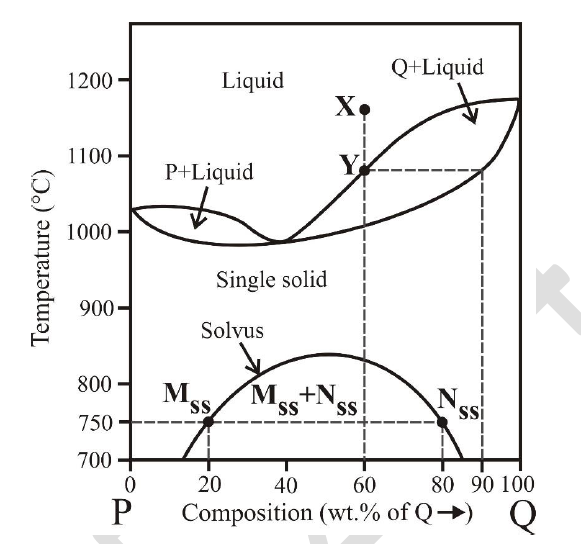
\includegraphics[width=0.6\columnwidth]{Figs/fig_8.png}
    \caption{Q.60.}
    \label{fig:q60}
\end{figure}
\begin{enumerate}
    \item Initial liquid composition is $60\,wt.\%$ of P and $40\,wt.\%$ of Q
    \item The composition of the solid in equilibrium with the liquid at 'Y' is $10\,wt.\%$ of P and $90\,wt.\%$ of Q
    \item The bulk composition of the final solid product is $40\,wt.\%$ of P and $60\,wt.\%$ of Q
    \item The proportion \brak{\text{on the basis of wt.\%}} of two phases, $M_{ss} \colon N_{ss}$ is $1 \colon 2 \text{ at } 750 \degree\,C$
\end{enumerate}
\hfill{\brak{\text{GATE GG 2025}}}

\item Which of the following statements is/are CORRECT for the M-plane of any fault?
\begin{enumerate}
    \item M-plane pole of a fault is located on the fault plane
    \item M-plane pole of a fault is perpendicular to the slickenline on the fault plane
    \item M-plane pole of a fault is parallel to the slickenline on the fault plane
    \item M-plane pole of a fault is perpendicular to the pole to the fault plane
\end{enumerate}
\hfill{\brak{\text{GATE GG 2025}}}

\item Which of the following microfossils is/are foraminifera?
\begin{enumerate}
    \begin{multicols}{4}
    \item Miliammina
    \item Triceratium
    \item Cibicides
    \item Guembelitria
    \end{multicols}
\end{enumerate}
\hfill{\brak{\text{GATE GG 2025}}}

\item The in situ stress at a point in a dry sandstone terrain is as follows: $\sigma_1 = 12\,MPa \text{ and } \sigma_3 = 4\,MPa$. The pore water pressure $\brak{p_w}$ increases by the construction of a reservoir. The failure criterion of the sandstone is given by $\sigma_1' = 3.48 MPa + 3\sigma_3'$, where $\sigma_1'$ and $\sigma_3'$ are the effective maximum and minimum principal stresses, respectively. Assuming that the failure occurs at peak stress, the minimum value of $p_w$ \brak{\text{in MPa}} that will cause the sandstone to fail in situ is \rule{3cm}{0.15mm} \brak{\text{rounded off to two decimal places}}.
\hfill{\brak{\text{GATE GG 2025}}}

\item If the $Rb-Sr$ isochron formed by a suite of gabbro samples has a slope of $0.0265$, then the calculated age of the gabbro in million years is \rule{3cm}{0.15mm} \brak{\text{in integer}}. [Use $\lambda\brak{^{87}\text{Rb}} = 1.42 \times 10^{-11}$ year$^{-1}$]
\hfill{\brak{\text{GATE GG 2025}}}

\item A soil mass comprises two horizontal layers \brak{\text{of equal thickness and equal width}} stacked one above the other. The hydraulic conductivities of the two layers are $5 \times 10^{-2}\,cm/s$ and $3 \times 10^{-2}\,cm/s$. Considering Darcian flow of water and same hydraulic gradient for both the layers, the effective hydraulic conductivity of the soil mass in $cm/s$ is \rule{3cm}{0.15mm} \brak{\text{rounded off to two decimal places}}.
\hfill{\brak{\text{GATE GG 2025}}}

\centering\section*{END OF THE QUESTION PAPER}

\end{enumerate}
\end{document}
